%
\let\textcircled=\pgftextcircled
\chapter{Theory}
\label{chap:theory}

\section{TODO}
\begin{enumerate}
    \item Add Bayesian estimation with priors
    \item explain disconnected sets
    \item Explain striding for Bayes
\end{enumerate}



\section{Introduction}
This chapter sets out the theory of Markov state models (MSMs) and hidden Markov models to describe the dynamics of biomolecular systems. Table \ref{tab:theory_nomenclature} summarises the  nomenclature used in this chapter. 

\begin{table}
    \centering
    \begin{tabular}{c|c}
        N & Number of atoms \\
        $\mathbf{x}/\mathbf{y}(t)$ & vector of $3N$ atomic coordinates as a function of time \\
        
        
    \end{tabular}
    \caption{Caption}
    \label{tab:theory_nomenclature}
\end{table}


\section{Markov processes}

Markov state models are now used routinely to quantitatively describe the conformational kinetics and thermodynamics of biomolecular systems using data collected from molecular dynamics (simulations) [] []. A single system is described by a vector of phase space (momentum and position) coordinates as a function of time, $\mathbf{x}(t)$, and ensemble of such systems can be described by a probability density over the same coordinates as a function of time, $p(\mathbf{x}; t)$. Modelling the system as a Markov process assumes that there exists a period of time, $\tau$, over which the evolution of the system from a point $\mathbf{x}(t)$ to a new point $\mathbf{y}(t+\tau)$ is dependent only on $\mathbf{x}(t)$, i.e. the joint probability density $p(\mathbf{x}, \mathbf{y} ; \tau)$ is conditional \emph{only} on $\mathbf{x}$:

\begin{equation}\label{eqn:markov_assumption}
p(\mathbf{x}, \mathbf{y} ; \tau)=\mathbb{P}[\mathbf{x}(t+\tau) \in \mathbf{y}+d \mathbf{y} | \mathbf{x}(t)=\mathbf{x}]
\end{equation}

In addition to the Markov property, equation \ref{eqn:markov_assumption}, three other assumptions are made when dealing with systems in thermodynamic equilibrium. First, the system is \emph{reversible} and so obeys detailed balance: 
\begin{equation}\label{eqn:detailed_balance}
\mu(\mathbf{x}) p(\mathbf{x}, \mathbf{y} ; \tau)=\mu(\mathbf{y}) p(\mathbf{y}, \mathbf{x} ; \tau), 
\end{equation}
in other words, the absolute probability of observing a transition from $\mathbf{x}$ to $\mathbf{y}$ (also known as the flux, $F(\mathbf{x}, \mathbf{y})$) is the same as that from $\mathbf{y}$ to $\mathbf{x}$. Second, there are no regions of phase space disconnected from one another, i.e. that the system is \emph{ergodic}. In this case there is a unique stationary distribution,  $\mu(\mathbf{x})$. Third, that the conditional probabilities in equation \ref{eqn:markov_assumption} are independent of time, i.e., the system is \emph{stationary}. 

The dynamics of the system under these assumptions is given by the \emph{transfer operator}, $\mathcal{T}(\tau)$, which propagates functions of the probability density: 
\begin{equation}\label{eqn:vector_norm}
    q(\mathbf{x} ; t) = p(\mathbf{x} ; t)/\mu(\mathbf{x}),
\end{equation}
forward in time by the following: 
\begin{equation}\label{eqn:transfer_operator}
\begin{split}
   q(\mathbf{y} ; t+\tau) &= \mathcal{T}(\tau) \cdot q(\mathbf{y} ; t) \\
   &=\frac{1}{\mu(\mathbf{y})} \int d \mathbf{x} p(\mathbf{x}, \mathbf{y} ; \tau) \mu(\mathbf{x}) q(\mathbf{x} ; t). 
\end{split}
\end{equation}

All the kinetic and thermodynamic information of the system is contained within $\mathcal{T}$, its eigenfunctions, $\psi_{i}(\mathbf{x})$, and eigenvalues $\lambda_{i}$. The eigenvalues lie within the interval $-1 < \lambda_i \le 1$ and the eigenvector/eigenvalue pairs shall be assumed to be ordered in decreasing value of $\lambda$. The first eigenvector, with $\lambda_{1}=1$, is equal to $\psi_{1}(\mathbf{x})=\mathbf{1}$. This corresponds to the stationary distribution $\mu(\mathbf{x})$ by virtue of the definition of $q(\mathbf{x}$, equation \ref{eqn:vector_norm}. 

The remaining eigenfunctions, $\psi_{2,3,4...}$, correspond to the relaxation processes which take the system from any initial distribution, $q(\mathbf{x} ; t=0)$ towards the stationary distribution on a timescale related to its corresponding eigenvalue. This can be seen by writing the time evolution of $u(\mathbf{x};t)$ as:

\begin{equation}\label{eqn:eig_decomp}
q(\mathbf{x} ; t+k \tau)=\mathbf{1}+\sum_{i=2}^{\infty} e^{-k \tau / t_{i}}\left\langle q(\mathbf{x} ; t), \psi_{i}(\mathbf{x})\right\rangle_{\mu} \psi_{i}(\mathbf{x}),
\end{equation}

where $k=1,2,3 \ldots$ is a time index, and $t_{i}=-\sfrac{\tau}{\ln{|\lambda_{i}|}}$ are the implied timescales for the relaxation process represented by $\psi_{i}(\mathbf{x})$. The bracketed quantity is the overlap between $q(\mathbf{x})$ and the eigenfunctions:

\begin{equation}
\left\langle q(\mathbf{x} ; t), \psi_{i}(\mathbf{x})\right\rangle_{\mu}=\int d \mathbf{x} \mu(\mathbf{x}) q(\mathbf{x} ; t) \psi_{i}(\mathbf{x})
\end{equation}

Each term in equation \ref{eqn:eig_decomp} will decay exponentially in the long time limit as $k \rightarrow \infty$, leaving just the first eigenvector, $\psi_{1}(\mathbf{x})=\mathbf{1}$, the stationary distribution. If the first $r$ eigenvalues are close to $1$ and are separated from the remaining values by a gap such that $\lambda_{r} \gg \lambda_{r+1}$, then its possible to truncate equation \ref{eqn:eig_decomp} without serious loss of accuracy to:

\begin{equation}\label{eqn:eig_decomp_to_r}
q(\mathbf{x},  t+k \tau)  \simeq \mathbf{1}+\sum_{i=2}^{r} e^{-k \tau / t_{i}}\left\langle q(\mathbf{x} ; t), \psi_{i}(\mathbf{x})\right\rangle_{\mu} \psi_{i}(\mathbf{x}).
\end{equation}

These $r$ eigenfunctions/eigenvalues are known as the \emph{dominant} eigenfunctions and they correspond to the slow relaxation processes of the system. The truncation amounts to describing just the slow kinetic processes of the system while ignoring the fast processes. This separation of timescales implies the existence of regions of phase space, partitioned by the dominant eigenfunctions, known as \emph{metastable} states. 

% This coarse-grained description becomes more accurate in the limit long time limit i.e. $k \tau \gg t_{m}$
% The sign structure of the dominant eigenvectors can be used to infer the location of metastable states within the phase space. To demonstrate how, we will use the 1 D four well potential which is shown in Figure $1 .$ Panel (b) shows the potential and panel (c) shows the normalized eigenvectors, $\psi_{i}(x) .$ The slowest relaxation process, $\psi_{2}(x),$ changes sign at $x=$ 0 clearly defining the boundary between the two sets of states separated by the highest potential barrier. Perron Cluster Cluster Analysis uses the two remaining dominant eigenvectors to partition the phase space (the $x$ axis) into four metastable states. This is shown in Figure $2 .$ The coloured lines in panel (b) show the probability that each point on the x axis belongs to one of four different metastable states. This is a fuzzy clustering of the $x$ axis.

% Prinz potential explainer here

\section{Markov state models}

Markov state models (MSMs) are discrete models of Markovian dynamics. The continuous quantities described above all have discrete analogues which will be described in detail in this section: 

\begin{itemize}
    \item The system is described by a set of $n$ discrete states labelled $1, \ldots, n$. Instead of the continuous vector $\mathbf{x}(t)$, each trajectory is denoted by a vector of integers $\mathbf{s}$. Each point in phase space is mapped to one of these states. 
    \item The system can be described by a probability mass vector, $\mathbf{p}(t)$  instead of a probability density function $p(\mathbf{x};t)$. The $i$th component of $\mathbf{p}(t)$ is the probability of the system being in  state $s_{i}$ at time $t$.
    \item The stationary distribution, $\bm{\pi}$, is defined using the continuous stationary distribution $\mu(\mathbf{x})$ and the definition of the discrete states: 
        \begin{equation}
            \pi_{i}=\int_{\mathbf{x} \in s_{i}} \mathrm{d}\mathbf{x}\mu(\mathbf{x})
        \end{equation}
    \item By analogy with equation \ref{eqn:vector_norm}, the system can also be described by $\mathbf{q}$ where $q_{i} = p_{i}/\pi_{i}$.
    \item The time evolution of $\mathbf{q}(t)$ and $\mathbf{p}(t)$ is determined by a the \emph{transition matrix}, $\mathbf{T}(\tau)$:
        \begin{align}
            \mathbf{q}(t+\tau) &= \mathbf{T}(\tau) \cdot \mathbf{q}(t) \\
            \mathbf{p}^{T}(t+\tau) & = \mathbf{p}^{T}(t)\cdot \mathbf{T}(\tau)
        \end{align}
    \item The eigenfunctions $\psi(\mathbf{x})$ are now the right eigenvectors of $\mathbf{T}(\tau)$, $\mathbf{v}$, with the same interpretation. The left eigenvectors, $\mathbf{u}$, are related to the right eigenvectors by: $u_{i} = v_{i}\cdot \pi_{i}$.  
 \end{itemize}

Creating an MSM starts with the collection of molecular dynamics (MD) data in the form of a set of short trajectories, with coordinates saved every $\Delta t$ seconds. Typically any bulk water molecules are ignored as are the momentum coordinates of all the atoms. If  each trajectory has $n_{\mathrm{f}}$ frames (coordinate snapshots) and $n_{\mathrm{a}}$ important atoms then trajectory is represented by a data matrix, $\mathbf{X} \in \mathbb{R}^{n_{\mathrm{f}} \times 3n_{\mathrm{a}}}$. 

The data then undergo a series of processing steps on the way to creating an MSM, these are: 

\begin{enumerate}
    \item \textbf{Create features:} A set of continuous features, $\chi_{i}, i \in \{1,\dots, n_{c} \}$ is created or chosen to represent the dynamics of the system:
    \begin{equation*}
        \mathbf{X}  \rightarrow \bm{\chi},\quad \bm{\chi} \in \mathbb{R}^{n_{f} \times n_{c}}
    \end{equation*}
    For example the feature might be the backbone dihedral angles of a peptide, or the contact distances between residues. 
    \item \textbf{Dimensionality reduction:} The number of features is reduced still further by transforming $\bm{\chi}$ into a small number, $m$, of collective variables. 
    \begin{equation*}
        \bm{\chi}  \rightarrow \bm{\chi}^{\prime},\quad \bm{\chi}^{\prime} \in \mathbb{R}^{n_{f} \times m}
    \end{equation*}
    This work will exclusively use time-lagged independent component analysis, TICA as a method of dimensionality reduction.  
    \item \textbf{Discretization:} Each of the MD frames is assigned to one of $n$ different discrete states using a clustering algorithm such as k-means clustering: 
    \begin{equation*}
        \bm{\chi}^{\prime} \rightarrow \mathbf{s},\quad \mathbf{s} \in \mathbb{Z}_{+}^{n_{f} \times 1}
    \end{equation*}
    \item \textbf{MSM estimation}: The transition matrix, $\mathbf{T}$, is estimated by counting transitions between discrete states separated by a time $\tau$. 
    \item \textbf{Coarse graining:} The MSM is then coarse-grained by lumping the $n$ microstates into $g$ macrostates states. This work will exclusively feature hidden Markov models (HMMs) as a method for doing this. 
\end{enumerate}

\subsection{Create features}
The choice of continuous feature $\chi$ may be determined (or strongly suggested) by the question being asked and/or from prior knowledge of the system. However, since the introduction of variational scoring rules such as the GMRQ [] and VAMP [], they are typically chosen using cross-validation. This is discussed in depth in chapter \ref{chap:msm}. 

\subsection{Dimensionality reduction with TICA}

Dimensionality reduction using TICA was introduced for improving MSM construction in [] and []. It is the result of variationally optimising a set of basis functions, $\chi_{i}$, to estimate the eigenfunctions, $\psi_{i}$, of the transfer operator. A detailed derivation is given in [] but can be summarised as follows. A trial function, $f$, is expanded in the basis $\chi_{i}$: 
\begin{equation}\label{eqn:trial_func}
    f(\mathbf{x}) = \sum_{i}a_{i}\chi_{i}(\mathbf{x})
\end{equation}
The variational principle for operators with bounded eigenvalues (such as the transfer operator) states that any approximate eigenfunction will have eigenvalues smaller than the true eigenvalues. So choosing the coefficients $a_{i}$ to maximize the eigenvalues from using equation \ref{eqn:trial_func} will be the closest approximation to the true eigenfunctions that can be achieved with linear combinations of basis functions. Using the method of Lagrange multipliers to maximize the eigenvalues using equation \ref{eqn:trial_func} results in the following generalized eigenvalue equation: \begin{equation}\label{eqn:general_ev_equation}
    \mathbf{C}\mathbf{a} = \lambda \mathbf{S}\mathbf{a}
\end{equation}
Solving this equation requires estimating the matrix elements of $\mathbf{C}$ and $\mathbf{S}$. The elements of $\mathbf{C}$ are the time-lagged correlation functions ($\mathbf{cor}$) between $\chi_{i}$ and $\chi_{j}$
\begin{equation}
    \begin{split}
        C_{ij} =& \operatorname{cor}\left(\chi_{i}, \chi_{j}, \tau\right)\\
        =& \int_{X} \int_{X} \chi_{i}(\mathbf{z}) \mathbb{P}\left(\mathbf{x}(t+\tau)=\mathbf{z} \mid \mathbf{x}(t)=\mathbf{y}\right) \\
        & \times \chi_{j}(\mathbf{y}) \mathbb{P}\left(\mathbf{x}(t)=\mathbf{y}\right) \mathrm{d} \mathbf{y} \mathrm{d}\mathbf{z},        
    \end{split}
\end{equation}
which can be estimated from the MD trajectories. The matrix $\mathbf{S}$ is the overlap matrix whose elements are the scalar product between the basis functions, weighted by the stationary distribution: 
\begin{align}
    S_{ij} &= \int \chi_{i}(\mathbf{x})\chi_{j}(\mathbf{x})\mu(\mathbf{x})^{-1} \mathrm{d}\mathbf{x}
\end{align}
Having solved for the TICA eigenvectors, keep the first $m$ columns of $\mathbf{a}$ and use this to transform feature matrix $\bm{\chi}$: 
\begin{equation}
    \bm{\chi}^{\prime} = \bm{\chi}\cdot[\mathbf{a}_{1}, \mathbf{a}_{2}, \cdots,  \mathbf{a}_{m}]
\end{equation}

\subsection{Discretization}
Discretization is performed on the $m$ dimensional feature matrix $\bm{\chi}$ using a clustering algorithm such as k-means or Ward clustering []. Each region of feature space, $S_{i}$, is assigned uniquely to the microstate $i$ through the associated indicator function, $s^{i}(\mathbf{x})$:
\begin{equation}
s^{i}(\mathbf{x})=\left\{\begin{array}{ll}
1, & \mathbf{x} \in S_{i} \\
0, & \mathbf{x} \notin S_{i}
\end{array}\right.
\end{equation}
To avoid introducing too many symbols, $s^{i}(\mathbf{x})$ denotes the indicator functions, while $\mathbf{s}$ is the MD trajectory in the indicator function basis. The individual components of $\mathbf{s}$ will be denoted $s_{t}$ where $t$ is a time index. To highlight the time series nature of $\mathbf{s}$ it will sometimes denoted $\{s_{1}, s_{2}, \ldots \}$. 

\subsection{MSM estimation}
MSM estimation is analogous to TICA estimation but with the indicator basis functions $s^{i}$ replacing the continuous basis functions $\chi_{i}$ in equation \ref{eqn:trial_func}. The result of the optimisation of coefficients $a_{i}$ results in the same generalized eigenvalue expression, equation \ref{eqn:general_ev_equation}. Solving this equation is simplified by the fact that the indicator functions are orthogonal and so $S_{ij} = 0$ if $i \neq j$ and $S_{ii} = \pi_{i}$, the discrete stationary distribution. Equation \ref{eqn:general_ev_equation} can be re-arranged to give: 
\begin{align}
 \mathbf{C a}=\lambda \bm{\Pi} \mathbf{a} \\
\mathbf{T a}=\lambda \mathbf{a}   
\end{align}
where $\bm{\Pi} = \mathrm{diag}\{pi_{1}, \ldots, \pi_{n}\}$ and $\mathbf{T}$, the transition matrix is $\mathbf{T} = \bm{\Pi}^{-1}\mathbf{C}$. In other words: 
\begin{equation}\label{eqn:tran_mat_def}
    T_{ij}(\tau) =\frac{\mathrm{cor}(s_{i}, s_{j}, \tau)}{\pi_{i}}
\end{equation}
The MSM estimation procedure consists of estimating the transition matrix elements which such that they respect the assumptions of i) reversibility and detailed balance, and ii) that the ergodicity i.e. that each state is connected to all other states. Two methods exist for estimating $T_{ij}$: maximum likelihood estimation, MLE, and Bayesian estimation. This work will make use of both: MLE will be used for model selection while Bayesian optimisation will be used when error estimates are required.  Detailed explanations of both  techniques can be found in [] but certain concepts need highlighting here: i) maximum likelihood estimation, ii) count matrices and ergodicity, iii) Bayesian estimation. 

\subsubsection{Maximum likelihood estimation}
Parameter estimation through maximum likelihood estimation proceeds by first modelling  the probability of observing the data $\{s_{1}, s_{2}, s_{3}, \ldots \}$ given \emph{fixed parameters}, $T_{ij}$. For a MSM  with  $\tau=1$ (in units of the trajectory time step, $\Delta t$) this is: 
\begin{equation}\label{eqn:msm_traj_like}
    \mathbb{P}(\mathbf{s}|\mathbf{T}) \propto \Pi_{t=1}^{n_{f}} T_{s_{t}, s_{t+1}}
\end{equation}
The likelihood, $\mathcal{L}(\mathbf{T}|\mathbf{s})$, is equal $\mathbb{P}(\mathbf{s}|\mathbf{T})$ but treats the the \emph{data as fixed} and the \emph{parameters as varying}\footnote{The integral of the likelihood over the parameter space can be greater $1$ hence it is not a probability}. The parameters which maximize $\mathcal{L}$ give a model with the best fit to the observed data. Equation \ref{eqn:msm_traj_like} can be re-written in terms of the count matrix, $c_{ij}$ (not the correlation matrix $C_{ij}$), which counts all the observed transitions between states $s_i$ and $s_j$: 
\begin{align}
    \mathcal{L}(\mathbf{T}|\mathbf{s}) & = \mathbb{P}(\mathbf{s}|\mathbf{T}) \\
    & \propto \Pi_{t=1}^{n_{f}} T_{s_{t}, s_{t+1}} \\ 
    & \propto \Pi_{i}\Pi_{j}T_{i, j}^{c_{ij}}. \label{eqn:msm_count_like}
    & = \mathbb{P}(\mathbf{c}|\mathbf{T})
\end{align}

\subsubsection{Count matrix}
As discussed in \cite{trendelkamp-schroerEstimationUncertaintyReversible2015b} the method for calculating the count matrix is important for estimating errors when  $\tau > 1\cdot \Delta t$. This is typically the case in molecular dynamics simulations as molecular motions are correlated at short times and MD frames can be recorded with almost arbitrary resolution.  The two extreme methods for counting are the \emph{sliding window} which over estimates the matrix elements and \emph{sample count} method which underestimates the matrix elements \cite{noeStatisticalInefficiencyMarkov}. \emph{Sliding window} counts all pairs of frames separated by $\tau$: $(s_1, s_{1+\tau}), (s_2, s_{2+\tau})$ etc. For example, a trajectory of $100$ frames with $\tau=2$ has $\sum_{i,j}c_{i,j}=98$. In this case, the confidence intervals generated will be too narrow due pairs of states separated by less than $\tau$ being correlated with each other and hence not independent. The \emph{sample count} method uses the only the states separated by $\tau$: $(s_1, s_{1+\tau}), (s_{1+\tau}, s_{1+2\tau})$ etc. continuing the example $\sum_{i,j}c_{i,j}=49$, a factor of $2$ different to the sliding window method. This leads to the confidence intervals being over-estimated. A third method, \emph{effective counting}, uses the sliding window method but scales each row of the count matrix by a different factor to account for correlation between the observations \cite{noeStatisticalInefficiencyMarkov}. Continuing the example, if the observations have low correlation, then the effective count matrix will be close the sliding window estimate; if the observations are highly correlated the count matrix will be closer to the sample count method. This method has been shown to give more accurate confidence intervals \cite{trendelkamp-schroerEstimationUncertaintyReversible2015b}. 

The count matrix, and therefore the method for counting,  will determine whether or not the states are ergodic. Two states, $i$ and $j$, are strongly connected if $c_{ij}, c_{ji}>0$ and the full set of states are said to be ergodic if they are strongly connected\cite{schererPyEMMASoftwarePackage2015a}. In all estimation procedures used in this work, if the full set of state are not strongly connected, then a subset of states are used such that all states within the subset are strongly connected.

\subsubsection{Bayesian estimation}\label{sec:theory_bayes}
Bayesian estimation \cite{gelmanBayesianDataAnalysis2014} uses not just the likelihood, $\mathbb{P}(\mathbf{c}|\mathbf{T})$, but the prior probability of the parameters themselves, $\mathbb{P}(\mathbf{T})$, to estimate the posterior probability of the parameters given the data, $\mathbb{P}(\mathbf{T}|\mathbf{c})$, through Bayes' rule: 
\begin{equation}
    \mathbb{P}(\mathbf{T}|\mathbf{c}) \propto \mathbb{P}(\mathbf{c}|\mathbf{T})\mathbb{P}(\mathbf{T})
\end{equation}
Rather than point estimates of the posterior, samples are drawn from the whole posterior distribution for each parameter, $T_{ij}$, using Markov chain Monte Carlo\cite{gelmanBayesianDataAnalysis2014}. These samples can then be used to estimate the distribution, and hence error, of any quantity determined by the transition matrix, e.g., eigenvalues or implied timescales. The details of the sampling procedures used for estimation of MSM in this work can be found in \cite{trendelkamp-schroerEstimationUncertaintyReversible2015b}, however two points should be highlighted here. First, the count matrix used are estimated using the effective count method. Second, the prior distribution for the transition matrix elements are defined over a reversible matrix $\mathbf{X}$, where $X_{ij}\propto T_{ij}\pi_{i}$, and is given by: 
\begin{equation}\label{eqn:theory_rev_prior}
    \mathbb{P}(\mathbf{X}) \propto \Pi_{i \ge j}x_{ij}^{-1}. 
\end{equation}
With this prior, the posterior transition matrix elements have the same connectivity structure as the count matrix. i.e. if $c_{ij}=0$ then for any posterior sample $T_{ij}=0$. 

To test the convergence of the sampling procedure to find stable values of the parameters, four independent sampling chains were produced and  the rank-normalized $\hat{R}$ statistic \cite{vehtariRanknormalizationFoldingLocalization2020}:
\begin{equation}
    \hat{R} = \frac{\hat{V}}{W}, 
\end{equation}
was calculated. Here $\hat{V}$ is the pooled variance of the four chains after rank normalization (i.e., sampled values are ranked and then the rank converted to a standard normal distributed variable) and $W$ is the within chain variance. Following the recommendations in \cite{vehtariRanknormalizationFoldingLocalization2020} the threshold value for convergence is $\hat{R} < 1.01$. 

\subsection{Choice of $\tau$}
The lag time, $\tau(\mathbf{MSM})$ is not a hyperparameter of the model but rather a part of the model specification; it defines the temporal resolution of the description of the dynamics. For large values of $\tau(\mathbf{MSM})$ the truncation of the dynamics to the dynamics of just the metastable states becomes more accurate. However, there may be processes of interest with timescales, $t_{i}<\tau(\mathrm{MSM})$ which will not be captured.

As a compromise, $\tau$ is chosen by inspection of the data by plotting the implied timescales [] as a function of $\tau(\mathrm{MSM})$.  Starting from a given discrete trajectory, $\{s_{t}\}$ estimate the largest implied timescale, $t_{2}$, for a range of different values of $\tau(\mathrm{MSM})$. Choose the smallest $\tau$ such that $\frac{d t_{2}}{d \tau} \simeq 0$. 

\subsection{Choice of hyperparameters}
The hyperparameters of the the MSM are the modelling choices which transform the raw MD data into the discrete states $s^{i}$ used in MSM estimation. This work will consider only the following parameters: 
\begin{enumerate}
    \item $\chi$ the continuous feature, 
    \item $\tau$ the TICA lag time, 
    \item $m$ the number of retained TICA components, 
    \item $n$ the number of cluster centers. 
\end{enumerate}
Other hyperparameters of the MSM fitting process will be kept fixed, these are: 
\begin{enumerate}
    \item The TICA eigenvectors will be scaled by their eigenvalues (``kinetic mapping'') so that euclidean distances in the TICA space will correspond to kinetic distances \cite{noeKineticDistanceKinetic2015}.
    \item the k-means algorithm will be used to cluster the TICA transformed trajectories. 
\end{enumerate}
Kinetic mapping is recommended for TICA dimensionality reduction \cite{noeKineticDistanceKinetic2015}, however, its utility in improving model performance is data set dependent \cite{husicOptimizedParameterSelection2016}.  Both k-means and Ward clustering have been shown to give good performance in MSMs \cite{husicWardClusteringImproves2017a}. Fixing both of these hyperparameters reflects an arbitrary decision to keep the number of hyperparameters to a minimum.

The hyperparameters are used to map the raw MD trajectories to the discrete MSM basis functions $s^{i}$. The variational principle, used previously to optimize the coefficients in the basis function expansion, equation \ref{eqn:trial_func}, can also be used to optimize the basis functions themselves \cite{schererVariationalSelectionFeatures2019}\cite{husicOptimizedParameterSelection2016}. In order to do this objective functions known as the VAMP (variational approach to Markov processes) scores \cite{wuVariationalApproachLearning2019} were derived which reach their upper limit when the resulting eigenfunctions become the exact eigenfunctions of the transfer operator. The VAMP scores were derived for both stationary and non-stationary, reversible and irreversible Markov processes and they generalize previous work on variationally optimising basis functions by \cite{mcgibbonVariationalCrossvalidationSlow2015} using the generalized matrix Rayleigh coefficient, GMRQ. The VAMP scores are a family of scores, parameterized by and integer $q$\cite{wuVariationalApproachLearning2019}: 
\begin{equation}\label{eqn:def_vampr}
\operatorname{VAMP}(q)=\sum_{i=1}^{r}\left(\lambda_{i}\right)^{q}, 
\end{equation} 
where $r$ is the number of dominant eigenvalues, $\lambda$, of the transition matrix (i.e. the $r$ in equation \ref{eqn:eig_decomp_to_r}). The GMRQ corresponds to $q=1$ and has been used to optimize parameters for MSMs of protein folding \cite{husicOptimizedParameterSelection2016}. This work will follow \cite{schererVariationalSelectionFeatures2019} which used the VAMP  score with $q=2$ (VAMP-2). 

In order to use the VAMP-2 score the following steps can be used:  \cite{schererVariationalSelectionFeatures2019}:
\begin{enumerate}
    \item select a set of hyperparameters to create a MSM basis, $s^{i}$, 
    \item estimate an MSM transition matrix, 
    \item calculate a VAMP-2 score, 
    \item repeat steps (1) - (3) a number of times until the VAMP-2 score converges. 
\end{enumerate}
However, using equation \ref{eqn:def_vampr}, will tend to produce complex basis functions that fit to noisy fluctuations in the data, rather than the `true' relaxation processes \cite{mcgibbonVariationalCrossvalidationSlow2015}\cite{wuVariationalApproachLearning2019}\cite{schererVariationalSelectionFeatures2019}, a process known as over-fitting \cite{friedman2001elements}.

Two popular techniques for mitigating over-fitting are the bootstrap [] and cross-validation (CV) \cite{friedman2001elements}. K-fold CV is popular for MSMs \cite{schererVariationalSelectionFeatures2019}\cite{mcgibbonVariationalCrossvalidationSlow2015} although many methods exist \cite{arlotSurveyCrossvalidationProcedures2009}. The idea of CV is to estimate the model parameters on a subset of the data, the training data $\mathcal{D}^{\mathrm{train}}$, and then evaluate the performance of the parameters on the remaining data $\mathcal{D}^{\mathrm{test}}$ \cite{friedman2001elements}. This work will use 50:50 shuffle split CV, which has been used previously in  \cite{chenDynamicConformationalLandscape2019}\cite{husicOptimizedParameterSelection2016}, and is described in algorithm \ref{alg:shuffle_split}. 

\begin{algorithm}\label{alg:shuffle_split}
\SetKwInput{Par}{Parameter}
\KwData{N independent trajectories: $\mathcal{D}=[\mathbf{s}_{1}, \mathbf{s}_{2}, \ldots, \mathbf{s}_{N}]$}
\KwData{hyperparameter set: $\theta$}
\KwData{estimator of model parameters: $P=P(\theta; \mathcal{D})$} 
\KwData{scoring function: $CV(\theta) = CV(P|\mathcal{D})$}
\Par{number of iterations: $J$}
\KwResult{Cross-validated score: $\operatorname{MCV}(\theta)$}
\BlankLine
\For{$i\leftarrow 1$ \KwTo $J$}{
    permute location of trajectories (``shuffle'') in $\mathcal{D}$: e.g., $\mathcal{D} \rightarrow [\mathbf{s}_{5}, \mathbf{s}_{17}, \ldots, \mathbf{s}_{2}]$\;
    split trajectories into two equal size, disjoint sets: $\mathcal{D} \rightarrow  \mathcal{D}^{\mathrm{train}},\quad \mathcal{D}^{\mathrm{test}}$\;
    estimate model parameters on training data: $P^{\mathrm{train}} = P(\theta,\mathcal{D}^{\mathrm{train}})$\;
    score model on test data: $CV^{\mathrm{test}}_{i} = CV_{i}(P^{\mathrm{train}}| \mathcal{D}^{\mathrm{test}})$\;
}
\KwResult{compute mean cross-validated score: $\operatorname{MCV}(\theta)=\frac{1}{J}\sum_{i}CV^{\mathrm{test}}(\theta)$}
\caption{50:50 shuffle split cross-validation}
\end{algorithm}
It is important to note that for CV to judge the performance of all the hyperparameters, the `estimator of model parameters' must take as its input the \emph{raw} data, \cite{friedman2001elements}. For the case of MSMs, the estimator takes the cartesian coordinates, applies TICA, clusters trajectories, and then estimates the transition matrix elements.  

The scoring function, $CV$, for the VAMP-2 score  \cite{wuVariationalApproachLearning2019} is given by: 
\begin{equation}
\operatorname{CV}\left(\mathbf{C}, \mathbf{S}, \mathbf{a} \mid \mathcal{D}_{\text {test }}\right) 
=\left\|\left(\mathbf{a}^{\top} \mathbf{S}^{\text{test}} \mathbf{a}\right)^{-\frac{1}{2}}\left(\mathbf{a}^{\top} \mathbf{C}^{\text{test}} \mathbf{a}\right)\left(\mathbf{a}^{\top} \mathbf{S}^{\text{test}} \mathbf{a}\right)^{-\frac{1}{2}}\right\|_{2}^{2}, 
\end{equation}
where the symbols retain their previous meaning and the $\left| A\right\|_{2}^{2}$ is the square of the Frobenius norm \cite{wuVariationalApproachLearning2019}. The matrices $\mathbf{S}^{\text{test}}$ and $\mathbf{C}^{\text{test}}$ are the overlap and correlation matrices estimated on the test data, while $\mathbf{a}$ are the eigenvectors of the transition matrix estimated using the training data. 

% To ensure the  measured response was generalisable \cite{friedman2001elements}, $20$ iterations of 50:50 shuffle split cross validation were used \cite{husicOptimizedParameterSelection2016}. For each trial this entailed fitting a model using \SI{50}{\percent} of the available data (the training data) with the following pipeline:

% \begin{enumerate}
%     \item \label{lst:modfititem1} The Cartesian coordinates were projected onto the required feature, $\chi$. 
%     \item \label{lst:modfititem2} For features (1) - (4) in AADH, TICA was applied with a lag time $\tau$ and the first $m$ independent  components were retained. 
%     \item \label{lst:modfititem3} k-means clustering \cite{friedman2001elements} was used to cluster the the frames in the TICA space into $n$ microstates.
%     \item \label{lst:modfititem4} A reversible, maximum likelihood Markov state model was estimated using these discrete trajectories. 
% \end{enumerate}

% The model was then scored on the remaining \SI{50}{\percent} (the test data) using the same pipeline without re-estimating the various model parameters (the expression for calculating the cross validated $\operatorname{VAMP}$ scores is described in \cite{mcgibbonVariationalCrossvalidationSlow2015} and \cite{wuVariationalApproachLearning2019}). This was repeated $20$ times, shuffling the trajectories in between each iteration [TM: Explain this].  The final trial response was calculated as the mean of the scores on the test data. All MSM fitting and MD trajectory analysis was performed in Python 3.7 using the packages PyEMMA \cite{schererPyEMMASoftwarePackage2015a}, MDTraj \cite{mcgibbonMDTrajModernOpen2015}, NumPy \cite{waltNumPyArrayStructure2011}, Pandas \cite{mckinneyPandasFoundationalPython2011}, Matplotlib \cite{hunterMatplotlib2DGraphics2007},  Seaborn \cite{michaelwaskomMwaskomSeabornV02020} and the Jupyter Project \cite{kluyverJupyterNotebooksPublishing2016} [TM: add version numbers].

% \subsubsection{Choice of $m$}
% With optimal choices of the hyperparameters and lag time the transition matrix represents a complete description of the dynamics of the system. In order to extract chemical significance from the transition matrix we must cluster the microstates into the metastable states of the system. This means:
% 1. choosing the number of metastable states deciding how many metastable states there are (the value of $m$ ) and;
% 2. assigning a probability for being in metastable state $i$ given we observe the system in state $s_{i}$, summarized in a membership matrix (equation 4-6).
% As with the choice of $s,$ pre-existing knowledge may constrain that choice but a simple data driven way of determining $m$ is to look at the ratio of successive eigenvalues ( $\lambda_{i} / \lambda_{i+1}$ ) or implied timescales $\left(t_{i} / t_{i+1}\right)$ and choose $m$ such that:
% \begin{equation}
% m=\arg \max \left(\frac{\lambda_{i}}{i_{i+1}}\right)
% \end{equation}

% This approach is ambiguous however, it may give different answers depending on whether $\lambda$ or $t$ are used and is susceptible to noise for small values of $\lambda$ or $t$ leading to large values of $m$. There may also be more than one plausible value of $m$ due to sampling error.
% There are a number of other ways of clustering the transition matrix which dictate the methods used to choose $m$. Clustering with PCCA provides two possible associated objective functions which can be used to select $m$ either on the full data or by using cross validation. These two functions either select for 'crispness' of the assignment (i:e. by trying to have as many 1s and 0s in $M_{i j}$ ) or for metastability.

% The other popular method for clustering the microstates is by estimating a hidden Markov model (HMM). $m$ can be selected using information criteria, bootstrapping and cross-validation and others. We will explore these more fully in chapter 3 .

\section{Coarse graining with Hidden Markov Models}\label{sec:theory_hmm}
\begin{figure}
    \centering
    \caption{\textbf{Hidden Markov model}}
    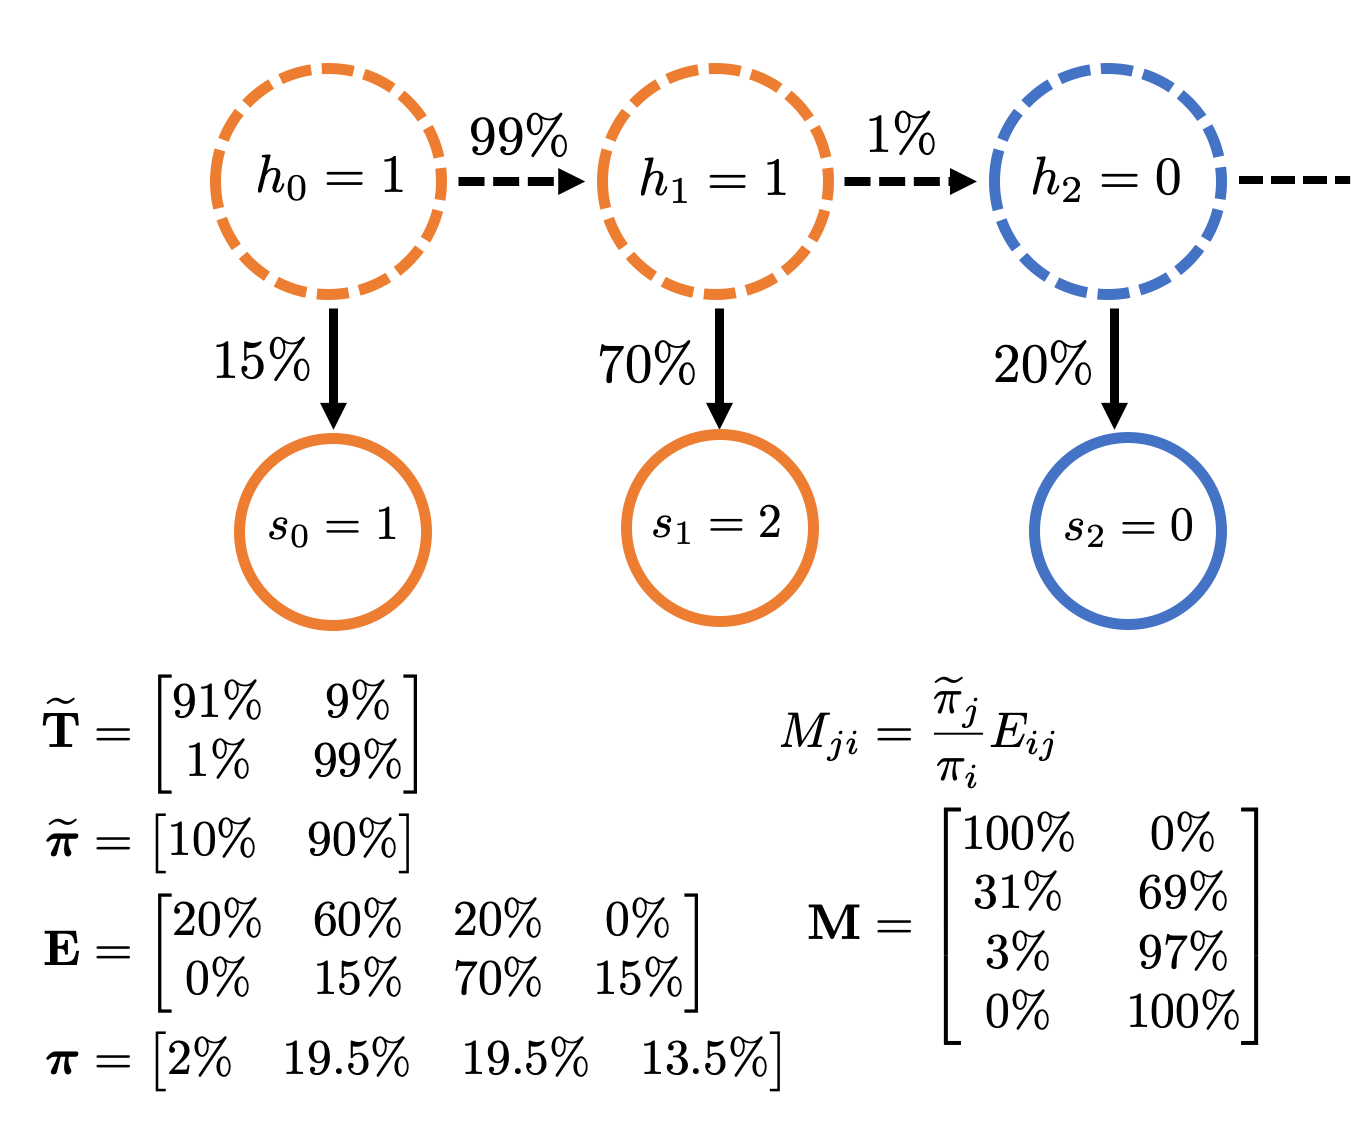
\includegraphics[width=0.8\textwidth]{chapters/theory/figures/hmm.png}
    \label{fig:theory_hmm}
\end{figure}
Hidden Markov models (HMMs) are models of a dynamic process consisting of the following elements\footnote{This treatment focuses exclusively on discrete hidden Markov processes.}\cite{rabinerTutorialHiddenMarkov1989}: 
\begin{enumerate}
    \item A number, $g$, of hidden states - these are not observed in the data used to train the model.  
    \item Hidden state to hidden state transition probabilities, $\mathbb{P}(h_{t+1}|h_{t})$, where $h_{t}$ is the hidden state at time $t$. These are encoded in the hidden state transition matrix, $\widetilde{\mathbf{T}}\in \mathbb{R}^{g \times g}$. This has the same interpretation as the MSM transition matrix.  
    \item A number, $n$ of observed states - these are the observations used to train the model. 
    \item Probabilities of observing the observed states, given a hidden state, encoded in the `emission matrix', $\mathbf{E}$, where  $E_{ij} = \mathbb{P}(s_t=j|h_t=i)$. 
    \item An initial distribution of states, $\widetilde{\bm{\pi}}$.
\end{enumerate}

An example HMM is shown in figure \ref{fig:theory_hmm}. The hidden states are shown in dashed circles with the state to state transition probability (the labelled dashed arrows) encoded in $\widetilde{T}$. The stationary distribution, $\widetilde{\bm{\pi}}$,  ensures detailed balance: $0.1\times 0.09 = 0.01\times 0.9$. While in each hidden state the system emits to a observed state (solid circles) with a probability (labelled solid arrows) encoded in the emission matrix $\mathbf{E}$. Other quantities of interest are the observed state stationary distribution $\bm{\pi}$, with $\pi_{j} = \sum_{i}E_{ij}\widetilde{\pi}_{i}$, and the membership matrix, $\mathbf{M}$. The membership matrix encodes the probability of the system being in an hidden state given the observed state \cite{noeProjectedHiddenMarkov2013a}, i.e., $M_{ji}=\mathbb{P}(h_t=j|s_t=i)$. This can determined from the stationary distributions of the hidden states and observed states, the emission matrix and the laws of probability: 
\begin{align}
    \mathbb{P}(h_t=i|s_j=j) &= \frac{\mathbb{P}(h_t=i)}{\mathbb{P}(s_t=j)}\mathbb{P}(s_j=j|h_t=i) \\
    M_{ji} &= \frac{\widetilde{\pi}_j}{\pi_i}E_{ij}
\end{align}

HMMs have been suggested as a method for modelling biomolecular dynamics by coarse graining a fitted MSM transition matrix\cite{noeProjectedHiddenMarkov2013a}. This coarse-graining is accurate under the following assumptions \cite{noeProjectedHiddenMarkov2013a}: 
\begin{enumerate}
    \item The underlying dynamics of the system are Markovian, i.e. they can be modelled by a transfer operator, equation \ref{eqn:}
    \item There is a gap between the $r$th and $r+1$th  eigenvalues of the underlying transfer operator. i.e. $\frac{\lambda_{r}}{\lambda_{r+1}} \gg 1$. The first $r$ eigenfunctions and eigenvalues are the \emph{dominant} set of eigenfunctions and eigenvalues. \label{assump_two}
    \item The $r$ dominant eigenfunctions decompose the stationary distribution into $r$ sets. The probability of the system being in the boundary between these sets is negligible. \label{assump_three}
\end{enumerate}
The process outlined in \cite{noeProjectedHiddenMarkov2013a} for coarse graining an MSM is as follows: 
\begin{enumerate}
    \item \textbf{Estimate an MSM}. Using the process outline in previous sections of this chapter transform the raw MD trajectories, $\mathbf{X}$, into trajectories of discrete states, $\mathbf{s}$. Using these discrete trajectories estimate the MSM transition matrix, $\mathbf{T}$. 
    \item \textbf{Determine number of metastable states}. The number of metastable states, $r$, is determined by looking for a gap in the eigenvalues of $\mathbf{T}$, such that  $\frac{\lambda_{r}}{\lambda_{r+1}} \gg 1$.
    \item \textbf{Coarse grain the transition matrix}. In order to estimate a HMM initial sets of the parameters, the matrices, $\widetilde{\mathbf{T}}_{0}$,  $\mathbf{E}_{0}$, and $\widetilde{\bm{\pi}}_{0}$ must be estimated. This is done using PCCA+ \cite{deuflhardRobustPerronCluster2005b} which clusters $\mathbf{T}$ into $r$ metastable states. The result of PCCA+ is the membership matrix, $\mathbf{M}$, from which values of the elements of $\widetilde{\mathbf{T}}_{0}$ and $\mathbf{E}_{0}$ can be estimated. 
    \item \textbf{Estimate the HMM}. The parameters of the model are updated and optimised from their initial values by maximizing likelihood estimation using the Baum-Welch[][] algorithm. 
\end{enumerate}

\begin{algorithm}\label{alg:baum_welch}
\DontPrintSemicolon
\SetKwInput{Par}{Parameter}
\KwData{Initial HMM parameters: $\theta_{0} = (\widetilde{\mathbf{T}}_{0}$,  $\mathbf{E}_{0}$, $\widetilde{\bm{\pi}}_{0})$}
\KwData{observed state trajectory: $\{s_t\}$, $t = 1, \ldots, N_{\mathrm{T}}$}
\Par{likelihood tolerance: $\epsilon$}
\BlankLine
\Begin{
$\mathrm{ll_{0}} \longleftarrow 0$\;
$\theta \longleftarrow \theta_{0}$\;
$\mathrm{C} \longleftarrow \mathtt{False}$\;
\While{$\mathrm{C}$}{
    \textbf{Forward procedure}\;
    Calculate the probability of being in hidden state $i$ at time $t$ and seeing the partial trajectory $s_1, \ldots, s_{t^{\prime}}$, given the model parameters:\;
    \begin{equation*}
      \alpha_i(t) = \mathbb{P}(\{s_{1}, \ldots, s_{t}\}| \theta)  
    \end{equation*}
    \textbf{Backward procedure}\;
    Calculate the probability of seeing the partial trajectory $s_{t+1}, \ldots, s_{N_{t}}$, given being in hidden state $i$ and the model parameters, $\theta$:\;
    \begin{equation*}
     \beta_i(t) = \mathbb{P}(\{s_{t+1}, \ldots, s_{N_{T}}\}|h_{t}=i, \theta)   
    \end{equation*}
    
    \textbf{Update model parameters}\;
    Calculate probability of being in hidden state $i$ at time $t$ given the entire trajectory $\{s_{t}\}$ and  $\theta$:\;
    \begin{equation*}
    \gamma_{i}(t) = \mathbb{P}(h_t=i|\{s_t\}, \theta) = \frac{\alpha_{i}(t) \beta_{i}(t)}{\sum_{j=1}^{g} \alpha_{j}(t) \beta_{j}(t)}
    \end{equation*}
    Calculate probability of begin in hidden state $i$ and time $t$ and transitioning to state $j$ at time $t+1$ given the entire trajectory $\{s_{t}\}$ and  $\theta$:\;
    \begin{equation*}
        \xi_{i,j}(t) = \mathbb{P}(h_t=i, h_{t+1} = j|\{s_t\}, \theta) = \frac{\alpha_{i}(t)T_{ij}\beta_{j}(t+1)E_{j, s_{t+1}}}{\sum_{k, l}^{g}\alpha_{k}(t)T_{kl}\beta_{l}(t+1)E_{l, s_{t+1}}}
    \end{equation*}
    \begin{align*}
        \widetilde{\pi}_{i}^{\prime}  &\longleftarrow \gamma_{i}(t=1) \\
        \widetilde{T}_{i,j}^{\prime} & \longleftarrow \frac{\sum_{t=1}^{N_{T}-1} \xi_{i j}(t)}{\sum_{t=1}^{N_{T}-1} \gamma_{i}(t)} \\
        E_{ij}^{\prime} & \longleftarrow \frac{\sum_{t=1}^{N_{T}} 1_{s_{t}=j} \gamma_{i}(t)}{\sum_{t=1}^{T} \gamma_{i}(t)} \\
        \theta & \longleftarrow (\widetilde{\bm{\pi}}^{\prime}, \widetilde{\mathbf{T}}^{\prime}, \mathbf{E}^{\prime})
    \end{align*}
    \textbf{Calculate log-likelihood}\;
    $\mathrm{ll}^{\prime} = \log{\left(\sum_{i}^{g}\alpha_{i}(N_{T})\right)}$\;
    \If{$\mathrm{ll}^{\prime}-\mathrm{ll} < \epsilon$}{
        $\mathrm{C} \longleftarrow \mathtt{True}$}
    $\mathrm{ll} \longleftarrow \mathrm{ll}^{\prime}$\;
}
}
\caption{The Baum-Welch algorithm}
\end{algorithm}

The Baum-Welch algorithm as used for coarse-graining reversible MSMs is given in detail in \cite{noeProjectedHiddenMarkov2013a}. The algorithm is sketched in algorithm \ref{alg:baum_welch} to introduce some of the important quantities used later in this thesis. In addition to the maximum likelihood estimation of the parameters, Bayesian estimation can be used, as described in section \ref{sec:theory_bayes}. A maximum likelihood HMM is used to initialise the parameters and set some of the prior distribution function parameters \cite{choderaBayesianHiddenMarkov2011a}. The prior functions used for the $\widetilde{\mathbf{T}}$ is the same as the MSM case (equation \ref{eqn:theory_rev_prior})and $\widetilde{\bm{\pi}}$ as implemented in the open source package PyEMMA (version 2.5.7) \cite{schererPyEMMASoftwarePackage2015a}:
\begin{equation}
    \widetilde{\bm{\pi}}_{0}  \sim \prod_{i} \widetilde{\pi}_{0, i}^{a_{i}+n_{i}-1} 
\end{equation}
where, $n_{i}$ is the number of times 



Needs much expansion!

Formula for striding interval $\Delta t_{\mathrm{s}}$ to decorrelate trajectories for Bayesian estimation. This is needed because the hidden states are not observed directly, so we can't adjust the count matrix as in the MSM case. Instead the trajectories are strided according to: 
\begin{equation}\label{eqn:hmm_striding}
    \Delta t_{\mathrm{s}} = \min{\left(\tau(\mathbf{MSM}), 2\cdot t_{g+1}\right)}
\end{equation}
$t_{g+1}$ slowest implied timescale (as measured by an MSM) which is then neglected in the HMM. i.e. if there are 5 hidden states in our required HMM these will hopefully correspond to the first 5 timescales (including $t_{1}=\infty$) in the full MSM basis. The 6th implied timescale measures in the MSM basis will the slowest relaxation timescale but which is nevertheless considered too fast to be included in the HMM. This timescale shouldn't be greater than $\tau$. 





\subsubsection{Model validation}\label{sec:model_validation}

Model validation is the process of checking how well the statistical model fits the data generating process. For protein dynamics we can ask ourselves: if we train a model, T, on some random sample of the protein dynamics, x, then how well does this We can assess the validity of a model either for the data in hand (in-sample, or internal validity) or for any future realisation of data (the out of sample or external validity. In the case of MSMs or HMMs we test whether the following relation holds:
$\mathbf{T}(k \tau) \simeq \mathbf{T}^{\mathbf{k}}(\tau)$
The lef-hand side is a transition matrix estimated with a lag time of $k r$ while the right-hand side is the matrix at time $\tau$ predicted from the matrix estimated with a lag of $\tau$. This equality will hold exactly for exact Markov process. For an $n \times n$ transition matrix, there will be $n^{2}$ comparisons to make which may become probibitivively computationally expensive. Instrad the comparison can be made for weighted combinations of microstates- the most natural combinations of microstates are the motestate and isble states This comparison is the Chappan-Kolmogorov (C-K) test

The C-K test equation 7 -1 holds by comparing the two terms for weighted combinations of the microstates. If a combination of microstates, $A$, is defined by a vector of $n$ weights, $w_{A}$, then the probability of being in that set at a time $k \tau$ later can be calculated in two ways:
LHS, equation 7 -1: using the counts of transitions from state $i$ to state $j$ in a given $k \tau, c_{i j}(k \tau)$ in the discretized trajectories:

\begin{equation}
p_{\text {trajectory }}(A, A: k r)=\sum_{k A}\left[w_{A i} \frac{\sum_{j \in A} c_{i}(k \tau)}{\sum_{i}^{N} c_{i j}(k \tau)}\right.
\end{equation}
RHS, equation 7-1: using the estimated transition matrix:

\begin{equation}
p_{\text {wsw }}(A, A, k \tau)=\sum_{\text {eft }}\left[w_{\tilde{1}}^{\top} \mathbf{k}^{\mathrm{k}}(\tau)\right]_{i}
\end{equation}

The Chapman-Kolmogorov test tests their equality:
\begin{equation}\label{eqn:ck_test}
p_{M S M}(A, A ; k \tau)=p_{\text {trajectory}}(A, A ; k \tau)
\end{equation}

The weights are typically the relevant columns of the membership matrix, i.e. $\left[w_{A}\right]_{i}=M_{i A}$
